\section{Security Protocols} % Message deduction?
Security protocols is an abstract or concrete protocol, that characterise the security related functions and applies cryptographic methods. It describes how the algorithm should be used to ensure the security and integrity of data transmitted. The security protocol is a protocol that runs in an untrusted environment, where it usually assumes channels are untrusted and participants are dishonest. In academic examples, they are often described with the Alice and Bob notation. (The Dolev-Yao model) 

A way of reason about wether a message is deductible by an adversary is through inference rules. Inference rules offers a formal analysis for proving security properties of protocols. \\ \\
TODO: discuss how Inference rules and derivation sequences can be used 


\subsection{Examples}
TODO: show examples of a man in the middle attack on the NS and DH protocols: \\ \\
- Needham-Schroeder Public key protocol (now modified according to Lowe's man in the middle attack): 
\begin{center}
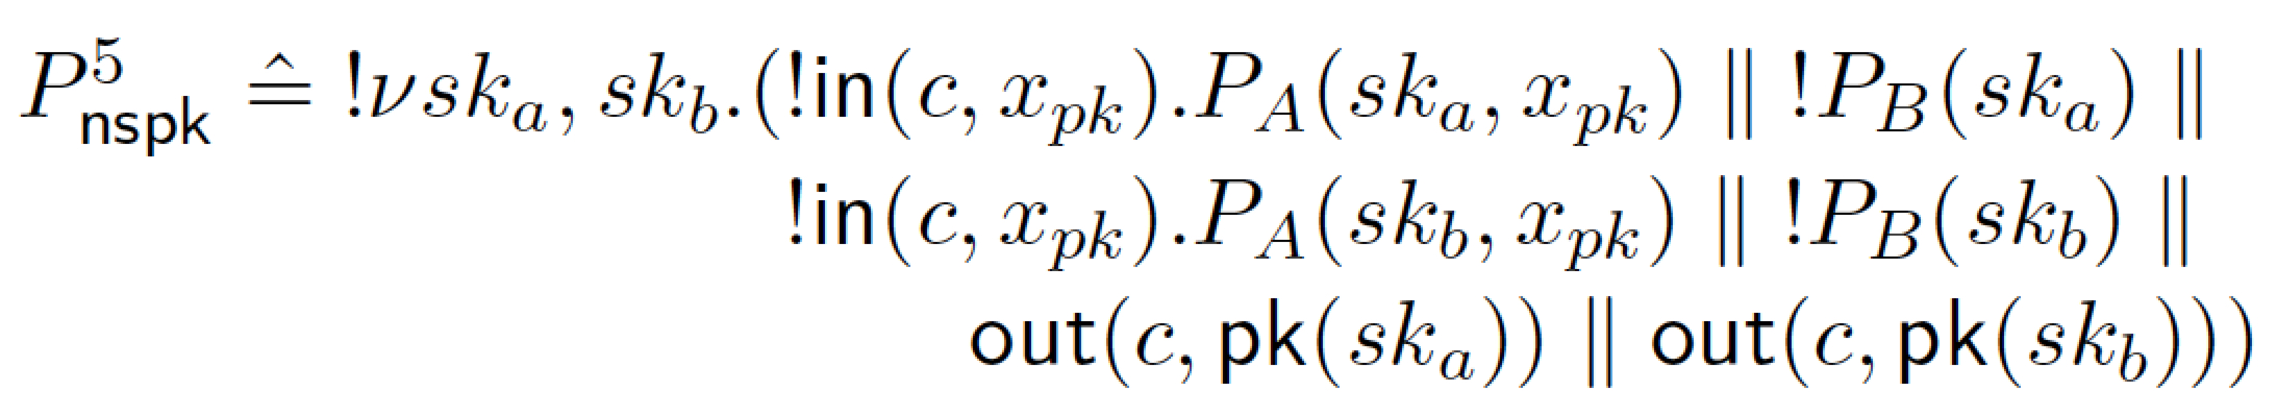
\includegraphics[width=0.7\textwidth, angle=0]{Graphics/Needham_Schroeder_Lowe.pdf}
\end{center}
- Diffie-Hellman protocol (man in the middle attack)

